\subsection{Broker}

We decided to put an intermediate broker between the middleware(s) and the
application server(s) to make our system more scalable.

Indeed, the messages sent by the middleware have two deficiencies:

\begin{enumerate}
  \item \textbf{Size:} middleware messages carry a significant amount of
    information, because middleware does not perform deep inspection of the
    payload (the application domain is completely transparent) and, therefore,
    messages are forwarded as they are received from the upper application
    layer;
  \item \textbf{Poor semantics:} middleware outputs events with its best
    effort, but it can only read the headers of application layer messages.
    Therefore, message topics are just a concatenation of little detailed
    information obtained by the application.
\end{enumerate}

Our message broker tries to overcome these problems by performing deep
inspection on the payloads of the messages, filtering information from them and
building more meaningful topics for the messages (we will provide more details
in Section \ref{sec:impl-broker}).


\subsubsection{Architecture}

The broker sub-system of our city simulator is written in Elixir, and leverages
Wabbit (a GenStage and RabbitMQ adapter).

A broker is basically a pipeline through which messages are processed:

\begin{itemize}
  \item \textit{BackendControlListener} : process which listens to
    a RabbitMQ instance shared
    with the middleware nodes,
    waiting for control messages;
  \item \textit{Daemon} :
    process which listens to
    a RabbitMQ instance shared
    with the middleware nodes,
    waiting for application-logic related messages;
  \item \textit{ContentEnricher} :
    process which elaborates middleware
    messages to augment their semantics,
    by adding domain-specific meta information;
  \item \textit{Forwarder} :
    process which puts messages
    on the output queues of a
    RabbitMQ broker
    shared with the application server.
\end{itemize}

A visual representation of this can be found in Figure \ref{fig:broker-arch}.

\begin{figure}[H]
  \centering
  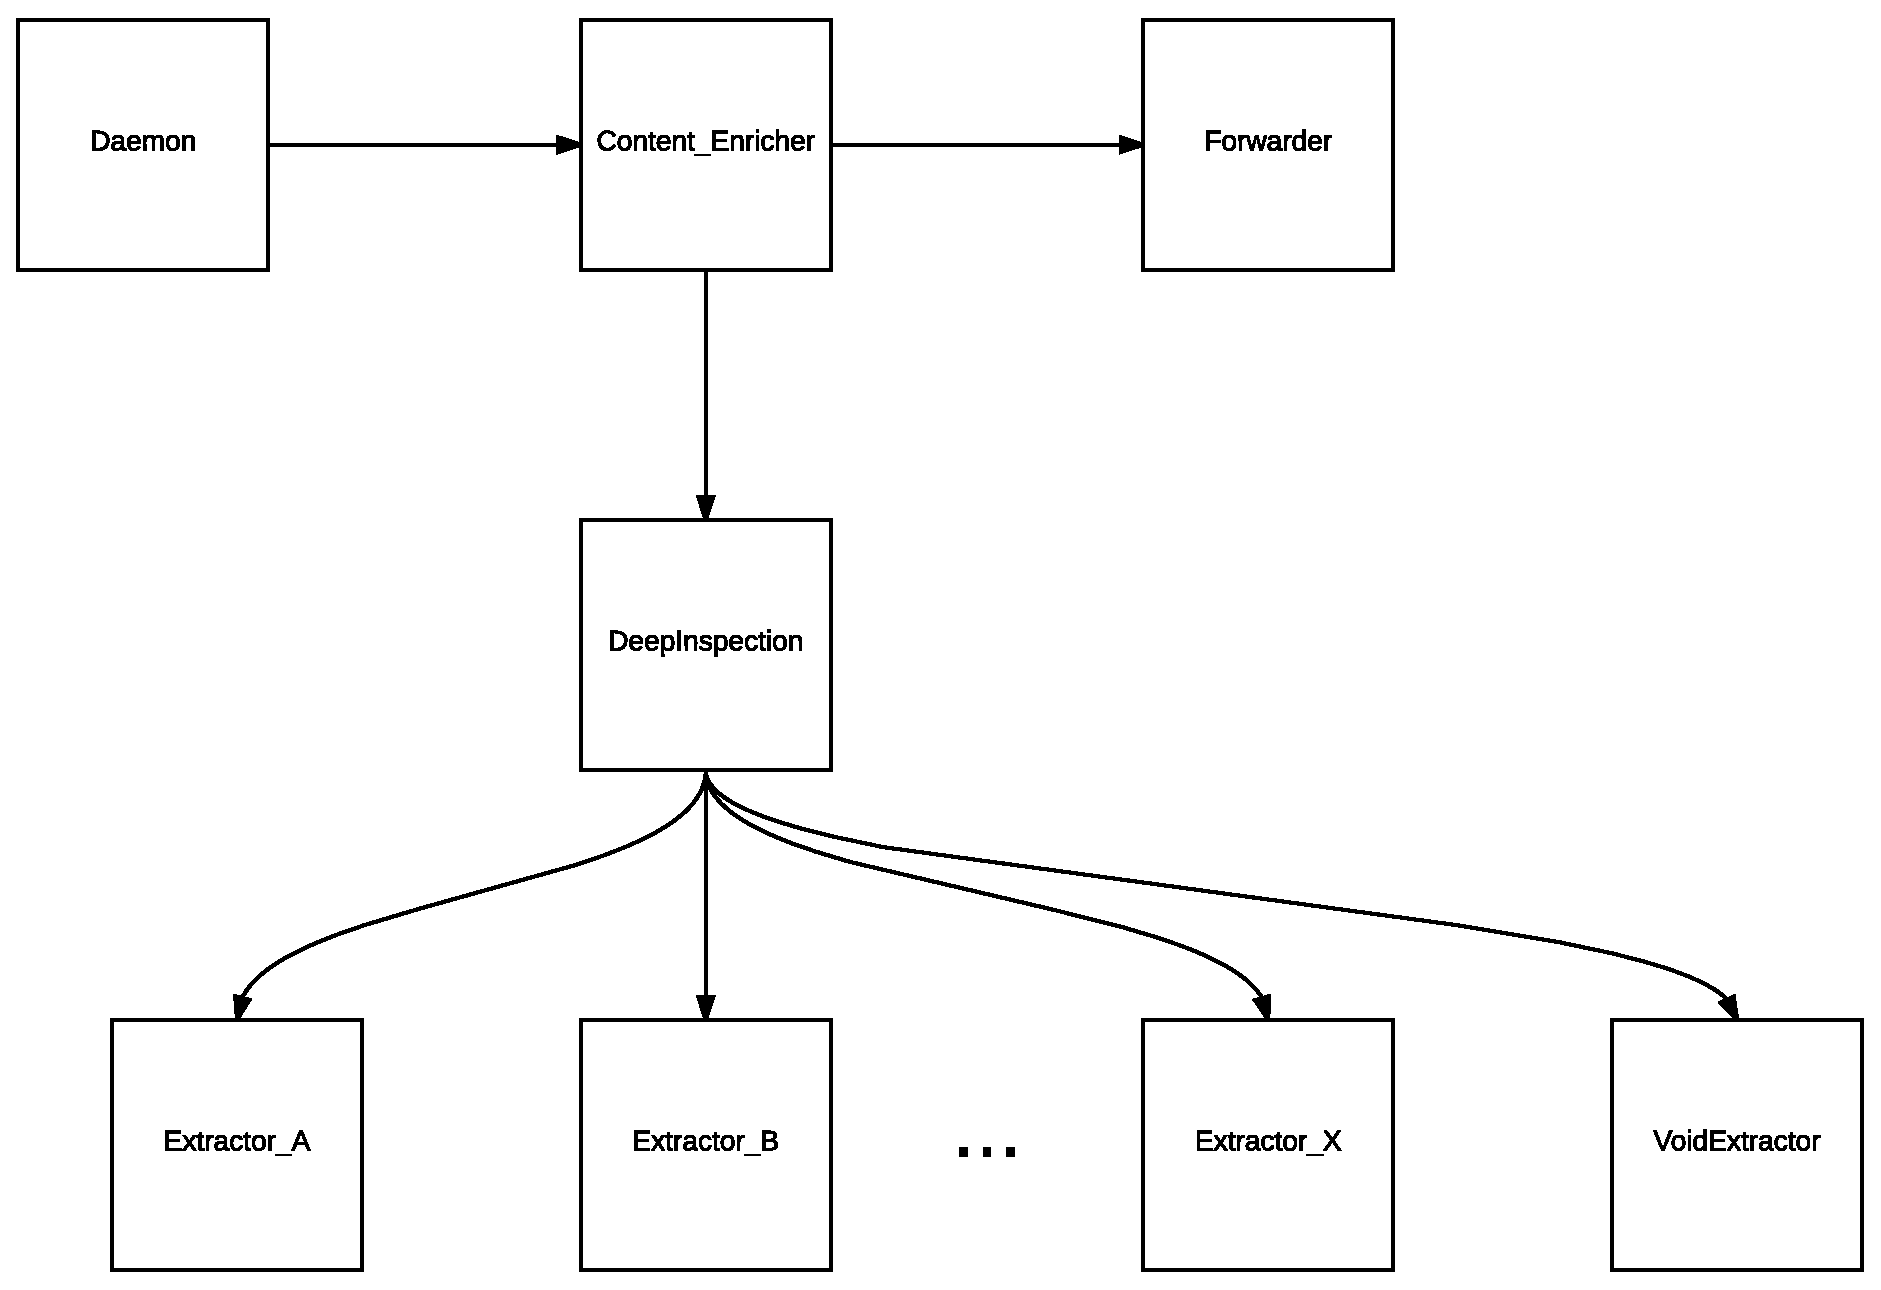
\includegraphics[width=.95\columnwidth]{images/implementation/broker.eps}
  \caption{Broker architecture}
  \label{fig:broker-arch}
\end{figure}

Clearly, each one of these processes could be arbitrarily replicated, for
instance we may decide to have 5 \textit{BackendControlListener}s, 3
\textit{Daemon}s, 6 \textit{ContentEnricher}s and 8 \textit{Forwarder}s, and
all of this would be fairly trivial to implement.

On the other hand, it is possible to spawn multiple copies of these
processes to deal with a increasing traffic load.
This might be done by evaluating the processes' demand and offer variables,
choosing some thresholds and spawning other supervised workers on demand.

Each \textit{ContentEnricher} is able to transform the  messages thanks to a
\textit{DeepInspection} module. Indeed, the latter inspects the message
to extract specific information.
It does so with the help of a series of Extractors modules\footnote{we did not
defined an Elixir Protocol, i.e., interface for them but it would have been
quite easy} which actuate the process. There is also a \textit{VoidExtractor}
module, which basically is a fallback case for an unidentified request.

\paragraph{Communication from frontend to backend}
Actually, our broker provides a means of communication from the frontend to
the backend as well.
We made this implementation choice because, even if it involves a flow of
information which goes in the opposite direction as the aforementioned
pipeline, we would have to instantiate another microservice to manage the
communication from the frontend to the backend.
Nevertheless, since at the moment the frontend contacts the backend only for
requiring a boot, we thought it was not meaningful to have a full-blown
microservice just for sending one control message, and we embodied
bi-directional communication into our broker.
